%\thispagestyle{myheadings}
\section{Keynote Address: Regina Barzilay}
\index{Barzilay, Regina}

\begin{center}
\begin{Large}
{\bfseries\Large How can NLP help cure cancer?}\vspace{1em}\par
\end{Large}

\daydateyear, 9:15--10:30 \vspace{1em}\\
Grande Ballroom \\
\vspace{1em}\par
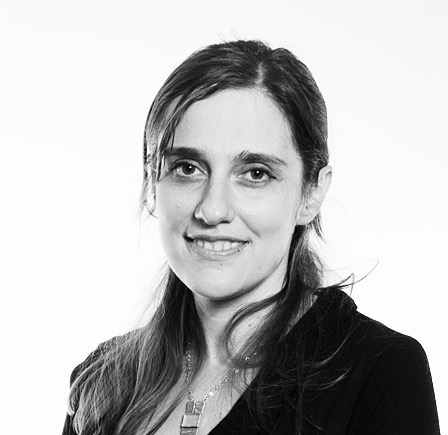
\includegraphics[height=100px]{content/day1/regina-hs-bw.jpg}
\end{center}

\noindent
{\bfseries Abstract} 

Cancer inflicts a heavy toll on our society. One out of seven women will 
be diagnosed with breast cancer during their lifetime, a fraction of them 
contributing to about 450,000 deaths annually worldwide. Despite billions 
of dollars invested in cancer research, our understanding of the disease, 
treatment, and prevention is still limited.

Majority of cancer research today takes place in biology and medicine. 
Computer science plays a minor supporting role in this process if at all. 
In this talk, I hope to convince you that NLP as a field has a chance to 
play a significant role in this battle. Indeed, free-form text remains the 
primary means by which physicians record their observations and clinical 
findings. Unfortunately, this rich source of textual information is 
severely underutilized by predictive models in oncology. Current models 
rely primarily only on structured data.

In the first part of my talk, I will describe a number of tasks where 
NLP-based models can make a difference in clinical practice. For example, 
these include improving models of disease progression, preventing 
over-treatment, and narrowing down to the cure. This part of the talk 
draws on active collaborations with oncologists from Massachusetts General 
Hospital (MGH).

In the second part of the talk, I will push beyond standard tools, 
introducing new functionalities and avoiding annotation-hungry training 
paradigms ill-suited for clinical practice. In particular, I will focus on 
interpretable neural models that provide rationales underlying their 
predictions, and semi-supervised methods for information extraction.

\vfill
\noindent
{\bfseries Biography}

Regina Barzilay is a professor in the Department of Electrical Engineering 
and Computer Science and a member of the Computer Science and Artificial 
Intelligence Laboratory at the Massachusetts Institute of Technology. Her 
research interests are in natural language processing. She is a recipient 
of various awards including of the NSF Career Award, the MIT Technology 
Review TR-35 Award, Microsoft Faculty Fellowship and several Best Paper 
Awards at NAACL and ACL. She received her Ph.D. in Computer Science from 
Columbia University, and spent a year as a postdoc at Cornell University.
\newpage
